\paragraph{Reliability: Concepts}

\begin{itemize}
\item Assume a computer has probability of failure {\color{red} p}
\item If the system needs {\color{orange} N } computers
  to work, what is the probability of
  system working?
\end{itemize}

\begin{itemize}
\item Probability of one component working: 1 - {\color{red} p}
\item Probability of all components working:
  $(1 - {\color{red} \text{p}})^{{\color{orange} \text{N}}}$
  \begin{itemize}
  \item assuming failures are independent!
  \item Correlated failures are the reality (and make it even worse)
  \end{itemize}
\end{itemize}


\paragraph{Reliability Measures}

\begin{itemize}
\item Mean Time to Failure ({\color{red} MTTF})
\item Mean Time to Repair ({\color{green} MTTR})
\item Mean Time Between Failures ({\color{blue} MTBF})
\item {\color{blue} MTBF} = {\color{red} MTTF} + {\color{green} MTTR}
\item Availability = {\color{red} MTTF} / {\color{blue} MTBF}
\item Downtime = (1 - Availability) =
  {\color{green} MTTR} / {\color{blue} MTBF}

\includegraphics[scale=0.15]{graphics/reliability-measures.png}

\item Consider {\color{orange} N = 10,000} and for one computer,
  {\color{red} MTTF = 30 years} then
  you have $10,000 / 30 \approx 333$ failures

\item In order to estimate the value of MTTF for
  a system that has long MTTF, run many machines simultaneously.
  This assumes that failures are evenly distributed during
  component lifetime.
\end{itemize}

\paragraph{Reliability \& Availability}
\begin{itemize}
\item Things will crash. Deal with it!
  \begin{itemize}
  \item Assume you could start with super reliable servers
    (MTBF of 30 years)
  \item Build computing system with 10 thousand of those
  \item \textbf{Watch one failure per day}
  \item Facebook has to mitigate one data center outage every
    two weeks!
  \end{itemize}
\end{itemize}

\begin{itemize}
\item {\color{brown} Fault-tolerant software is inevitable}
\end{itemize}

\begin{itemize}
\item Typical yearly flakiness metrics
  \begin{itemize}
  \item 1-5\% of your disk drives will die
  \item Servers will crash at least twice (2-4\% failure rate)
  \end{itemize}
\end{itemize}


\paragraph{Faults, Errors, and Failures}
\begin{itemize}
\item \textbf{Fault}
  \begin{itemize}
  \item Defect that has potential to cause problems
  \end{itemize}

\item \textbf{Error}
  \begin{itemize}
  \item Wrong result caused by an active fault
  \end{itemize}

\item \textbf{Failure}
  \begin{itemize}
  \item Unhandled error that causes interface to break its contract
  \end{itemize}
\end{itemize}

\paragraph{Fault Tolerance}
\begin{itemize}
\item Error detection
  \begin{itemize}
  \item Use limited redundancy to verify correctness
  \item Example: detect damaged frames in link layer
  \item \textbf{Fail fast:} report error at interface
  \end{itemize}
\end{itemize}

\begin{itemize}
\item Error containment
  \begin{itemize}
  \item Limiting propagation of errors
  \item Example: enforced modularity
  \item \textbf{Fail stop:} immediately stop to prevent propagation
  \item \textbf{Fail safe:} transform wrong values into
    conservative ``acceptable'' values, but limiting operation
  \item \textbf{Fail soft:} continue with only a subset of
    functionality
  \end{itemize}
\end{itemize}

\paragraph{Fault Tolerance}
\begin{itemize}
\item Error masking
  \begin{itemize}
  \item Ensure correct operation despite errors
  \item Example: reliable transmission, process pairs
  \end{itemize}

\item We will focus on error masking
  \begin{itemize}
  \item Main techniques: \textbf{Redundancy}
  \end{itemize}
\end{itemize}

\paragraph{Replication}
\begin{itemize}
\item State-machine replications (replicated Interpreter)
\item Asynchronous replication (replicated memory)
  \begin{itemize}
  \item Primary-Site
  \item Peer-to-Peer
  \end{itemize}

\item Synchronous replication (replicated memory)
  \begin{itemize}
  \item Read-Any, Write-All
  \item Quorums
  \end{itemize}
\end{itemize}

\begin{itemize}
\item Techniques only good enough for a specific \textbf{failure model}
  \begin{itemize}
  \item Nuclear holocaust
  \item Component maliciously outputs random gibberish
    (\textbf{Byzantine})
  \item Components \textbf{crash} without telling you anything
  \item Components are \textbf{fail-stop}
  \end{itemize}
\end{itemize}

\paragraph{Asynchronous Replication}
\begin{itemize}
\item Allows WRITEs to return before all copies have been changed
  \begin{itemize}
  \item READs nonetheless look at subset of copies
  \item Users must be aware of which copy they are reading,
    and that copies may be out-of-sync for short periods of time
  \end{itemize}
\end{itemize}

\begin{itemize}
\item Two approaches: Primary Site and Peer-to-Peer replication
  \begin{itemize}
  \item Difference lies in how many copies are ``updatable''
    or ``master copies''
  \end{itemize}
\end{itemize}

\paragraph{Primary Site Replication}
\begin{itemize}
\item Exactly one copy is designated the primary or master copy.
  Replicas at other sites cannot be directly updated
  \begin{itemize}
  \item The primary copy is published
  \item other sites subscribe to this copy; these are secondary copies
  \end{itemize}
\end{itemize}

\begin{itemize}
\item Main issue: How are changes to the primary copy propagated to the
  secondary copies?
  \begin{itemize}
  \item Done in two steps: First, CAPTURE changes made at primary;
    then APPLY these changes
  \item Many possible implementations for CAPTURE and APPLY
  \end{itemize}
\end{itemize}

\paragraph{Primary copy}

\includegraphics[scale=0.15]{graphics/primary-copy.png}

\begin{itemize}
\item Writers lock \& update primary copy and propagate the
  update to other copies
\item Readers lock and access primary copy
\item Widely adopted, e.g. many database systems
\end{itemize}


\paragraph{Peer-to-Peer Replication}
\begin{itemize}
\item More than one of the copies of an object can be a master in
  this approach
  \begin{itemize}
  \item Changes to a master copy must be propagated to to other copies
  \item It two master copies are changed in a conflicting
    manner, this must be resolved. (e.g., Site 1: Joe's
    age changed to 35; Site 2: to 36)
  \end{itemize}
\end{itemize}

\begin{itemize}
\item Best used when conflicts do not arise
\item \textbf{Examples}
  \begin{itemize}
  \item Each master site owns a disjoint fragment of the data
  \item Updating rights owned by one master at a time
  \item Operations are associative-commutative
  \end{itemize}
\end{itemize}

\paragraph{Eventual consistency}
\begin{itemize}
\item If no new updates are made to an object, after some
  inconsistency window closes, all accesses will return the
  same ``last'' updated value
\end{itemize}

\begin{itemize}
\item \textbf{Prefix property:}
  \begin{itemize}
  \item If Host 1 has seen write $w_{i,2}: i^{th}$ write accepted
    by host 2
  \item Then 1 has all writes $w_{j,2}$ (for $j < i$) accepted
    by 2 prior to $w_{i,2}$
  \end{itemize}
\end{itemize}

\begin{itemize}
\item Assumption: write conflicts will be easy to resolve
  \begin{itemize}
  \item Even easier if whole-''object'' updates only
  \end{itemize}
\end{itemize}

\paragraph{Events and Histories}
\begin{itemize}
\item Processes execute sequences of events

\item Events can be of 3 types:
  \begin{itemize}
  \item local
  \item send
  \item receive
  \end{itemize}

\item The local history $h_p$ of process p is the sequence of
  events executed by process
\end{itemize}

\paragraph{Ordering Events}
\begin{itemize}
\item Observation 1:
  \begin{itemize}
  \item Events in local history are \textbf{totally ordered}
  \end{itemize}

  \includegraphics[scale=0.15]{graphics/order-events-obs-1.png}

\item Observation 2:
  \begin{itemize}
  \item For every message m, send(m) precedes receive(m)
  \end{itemize}

  \includegraphics[scale=0.15]{graphics/order-events-obs-2.png}

\end{itemize}

\paragraph{Happens-Before (Lamport [1978])}
\begin{itemize}
\item Relative time? Define Happens-Before (→):
  \begin{itemize}
  \item On the same process: {\color{blue} a → b, if time(a) < time(b)}
  \item If p1 sends m to p2: {\color{blue} send(m) → receive(m)}
  \item Transitivity: {\color{blue} If a → b and b → c then a → c}
  \end{itemize}
\end{itemize}

\begin{itemize}
\item Lamport Algorithm establishes partial ordering:
  \begin{itemize}
  \item All processes use counter (clock) with initial value of 0
  \item Counter incremented / assigned to each event as timestamp
  \item A send (msg) event carries its timestamp
  \item For receive (msg) event, counter is updated by \\
    {\color{blue} max (receiver-counter, message-timestamp) + 1}
  \end{itemize}
\end{itemize}


\paragraph{Lamport Logical Time}

\includegraphics[scale=0.15]{graphics/lamport-logical-time.png}

Problem:

\includegraphics[scale=0.15]{graphics/lamport-problem.png}


\paragraph{Vector Logical Clocks}

\begin{itemize}
\item \textbf{With Lamport Logical Time}
  \begin{itemize}
  \item e precedes f ⇒ timestamp(e) < timestamp(f), but
  \item timestamp(e) < timestamp(f) $\centernot\Rightarrow$
    e precedes f
  \end{itemize}
\end{itemize}

\begin{itemize}
\item \textbf{Vector Logical time} guarantees this:
  \begin{itemize}
  \item All hosts use a vector of counters (logical clocks),
  \item $i$-th element is the clock value for host $i$, initially 0
  \item Each host $i$, increments the $i$-th element of its vector
    upon an event, assigns the vector to the event
  \item A send(msg) event carries vector timestamp
  \item For receive(msg) event:
\begin{align*}
    \text{V}_{\text{receiver}}[j] = \begin{cases}
      \max (\text{V}_{\text{receiver}}[j], \text{V}_{\text{msg}}[j]),
      \quad \text{if \textit{j} is not self} \\
      \text{V}_{\text{receiver}}[j] + 1
      \hspace{1.8cm} \text{otherwise}
      \end{cases}
\end{align*}
  \end{itemize}
\end{itemize}

\paragraph{Example: Vector Logical Time}
\includegraphics[scale=0.15]{graphics/ex-vector-logical-time.png}


\paragraph{Comparing Vector Timestamps}
\begin{itemize}
\item a = b \hspace{0.5cm} if they agree at every element
\item a < b \hspace{0.5cm} if a[i] <= b[i], for every i, but !(a=b)
\item a > b \hspace{0.5cm} if a[i] >= b[i], for every i, but !(a=b)
\item a || b \hspace{0.5cm} if a[i] < b[i], a[j] > b[j], for some i,j
  \textbf{(conflict!)}
\end{itemize}

\begin{itemize}
\item If one history is prefix of other, then one vector
  timestamp < other
\item If one history is not a prefix of the other, then
  (at least by example) VTs will not be comparable
\end{itemize}

\paragraph{Eventual is not the only choice}
\begin{itemize}
\item Host of other properties available
  (beyond the scope of this course!)
\item Examples:
  \begin{itemize}
  \item Strong consistency
  \item Weak consistency
  \item Causal consistency
  \item Read-your-writes consistency
  \item Session consistency
  \item Monotonic read consistency
  \item Monotonic write consistency
  \end{itemize}
\end{itemize}

\paragraph{Synchronous Replication}
\begin{itemize}
\item Hide replication behind READ/WRITE memory abstraction
\item Program operates against memory
\item Memory makes sure READs and WRITEs are \textbf{atomic}
  \begin{itemize}
  \item \textbf{All-or-nothing:} either in all correct replicas or none
  \item \textbf{Before-or-after:} Equivalent to a total order
  \end{itemize}
\item Memory replicates data for fault tolerance
\end{itemize}

\paragraph{Read Any, Write-All}

\begin{itemize}
\item For now assume we have a centralized Dispatcher
  → state-machine replication algorithms drop that assumption!
\item WRITEs synchronously sent everywhere
\item But READs can be answered by any replica
\end{itemize}

\includegraphics[scale=0.15]{graphics/read-any-write-all.png}

\paragraph{Quorums}
\begin{itemize}
\item Read Quorum ($\text{Q}_r$) / Write Quorum ($\text{Q}_W$)
\item $\text{Q}_r$ + $\text{Q}_W$ > $\text{N}_{\text{replicas}}$
\item Reads or writes only succeed if same response is given by
  respective quorum
  \begin{itemize}
  \item Read any, Write all case is
    $\text{Q}_W$ = $\text{N}_{\text{replicas}}$, $\text{Q}_r = 1$
  \end{itemize}
\end{itemize}

% LocalWords:  MTTF MTTR MTBF Unhandled modularity WRITEs READs th
% LocalWords:  updatable Lamport msg VTs
